\documentclass[12pt,letterpaper]{article}
\usepackage{graphicx,textcomp}
\usepackage{natbib}
\usepackage{setspace}
\usepackage{fullpage}
\usepackage{color}
\usepackage[reqno]{amsmath}
\usepackage{amsthm}
\usepackage{fancyvrb}
\usepackage{amssymb,enumerate}
\usepackage[all]{xy}
\usepackage{endnotes}
\usepackage{lscape}
\newtheorem{com}{Comment}
\usepackage{float}
\usepackage{hyperref}
\newtheorem{lem} {Lemma}
\newtheorem{prop}{Proposition}
\newtheorem{thm}{Theorem}
\newtheorem{defn}{Definition}
\newtheorem{cor}{Corollary}
\newtheorem{obs}{Observation}
\usepackage[compact]{titlesec}
\usepackage{dcolumn}
\usepackage{tikz}
\usetikzlibrary{arrows}
\usepackage{multirow}
\usepackage{xcolor}
\newcolumntype{.}{D{.}{.}{-1}}
\newcolumntype{d}[1]{D{.}{.}{#1}}
\definecolor{light-gray}{gray}{0.65}
\usepackage{url}
\usepackage{listings}
\usepackage{color}

\definecolor{codegreen}{rgb}{0,0.6,0}
\definecolor{codegray}{rgb}{0.5,0.5,0.5}
\definecolor{codepurple}{rgb}{0.58,0,0.82}
\definecolor{backcolour}{rgb}{0.95,0.95,0.92}

\lstdefinestyle{mystyle}{
	backgroundcolor=\color{backcolour},   
	commentstyle=\color{codegreen},
	keywordstyle=\color{magenta},
	numberstyle=\tiny\color{codegray},
	stringstyle=\color{codepurple},
	basicstyle=\footnotesize,
	breakatwhitespace=false,         
	breaklines=true,                 
	captionpos=b,                    
	keepspaces=true,                 
	numbers=left,                    
	numbersep=5pt,                  
	showspaces=false,                
	showstringspaces=false,
	showtabs=false,                  
	tabsize=2
}
\lstset{style=mystyle}
\newcommand{\Sref}[1]{Section~\ref{#1}}
\newtheorem{hyp}{Hypothesis}


\title{Problem Set 4}
\date{Due: December 3, 2023}
\author{Applied Stats/Quant Methods 1}


\begin{document}
	\maketitle
	\section*{Instructions}
	\begin{itemize}
		\item Please show your work! You may lose points by simply writing in the answer. If the problem requires you to execute commands in \texttt{R}, please include the code you used to get your answers. Please also include the \texttt{.R} file that contains your code. If you are not sure if work needs to be shown for a particular problem, please ask.
		\item Your homework should be submitted electronically on GitHub.
		\item This problem set is due before 23:59 on Sunday December 3, 2023. No late assignments will be accepted.
	\end{itemize}



	\vspace{.5cm}
\section*{Question 1: Economics}
\vspace{.25cm}
\noindent 	
In this question, use the \texttt{prestige} dataset in the \texttt{car} library. First, run the following commands:

\begin{verbatim}
install.packages(car)
library(car)
data(Prestige)
help(Prestige)
\end{verbatim} 


\noindent We would like to study whether individuals with higher levels of income have more prestigious jobs. Moreover, we would like to study whether professionals have more prestigious jobs than blue and white collar workers.

\newpage
\begin{enumerate}
	
	\item [(a)]
	Create a new variable \texttt{professional} by recoding the variable \texttt{type} so that professionals are coded as $1$, and blue and white collar workers are coded as $0$ (Hint: \texttt{ifelse}).
	
	\vspace{1cm}
	
	\lstinputlisting[language=R, firstline=1, lastline=20]{PS04_my_answers_daijin_zhou.R}
	
	
	\item [(b)]
	Run a linear model with \texttt{prestige} as an outcome and \texttt{income}, \texttt{professional}, and the interaction of the two as predictors (Note: this is a continuous $\times$ dummy interaction.)
	
	\vspace{1cm}
	\lstinputlisting[language=R, firstline=21, lastline=42]{PS04_my_answers_daijin_zhou.R}
	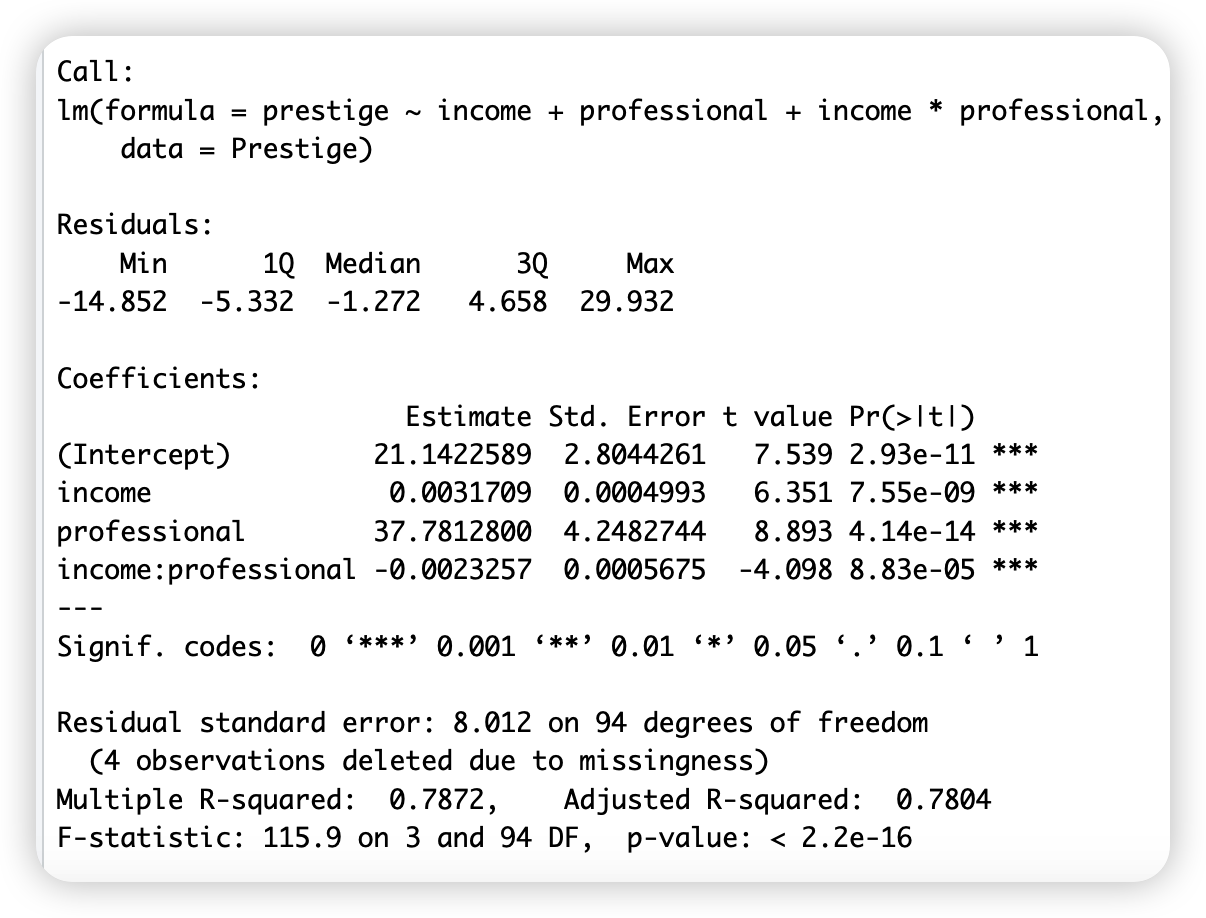
\includegraphics[width=0.99\textwidth]{1-2.png}
	\noindent
	Interpretation:\\
	Check the significance of coefficients: from the summary of the regression model, the P-values of the coefficients are both less than 0.05 , so the coefficients are statistically significant.\\
	
	So, The regression model is: \\
	y-hat-prestige = 21.14226 + 0.0032*income + 37.7812*professional - 0.0023*income*professional
	\item [(c)]
	Write the prediction equation based on the result.\\
	\noindent
	
	Interpretation:\\
	Prediction equation for professionals (professional = 1):\\
	
	y-hat = 21.1422 + 0.0032*income + 37.7812*professional - 0.0023*income*professional\\
	y-hat-1 = 21.1422 + 0.0032*income + 37.7812*1 - 0.0023*income*1 \\
	
	So, the prediction equation for professionals is : \\
	y-hat-1 = 58.9234 + 0.0009*income\\
	
	\noindent
	Prediction equation for non-professionals/Blue Collar and white Collar(professional = 0):\\
	
	y-hat = 21.1422 + 0.0032*income + 37.7812*professional - 0.0023*income*professional\\
	y-hat-0 = 21.1422 + 0.0032*income + 37.7812*0 - 0.0023*income*0\\
	
	So, the prediction equation for non-professionals is : \\
	y-hat-0 = 21.1422 + 0.0032*income\\

\newpage
	\item [(d)]
	Interpret the coefficient for \texttt{income}.
	
	\vspace{1cm}	
	\noindent
	Interpretation:\\
	Income effect for professionals:\\
	For professionals, with every additional 1 USD of income, the average increase of Prestige is 0.0009.\\
	
	Income effect for non-professionals:\\
	For non-professionals, with every additional 1 USD of income, the average increase of Prestige is 0.0032.\\
	\item [(e)]
	Interpret the coefficient for \texttt{professional}.\\
	\noindent
	
	Interpretation:\\
	Rearrange the regression model: \\
	y-hat = 21.1422 + 37.7812*professional +(0.0032-0.0023*professional)*income\\
	
	When the income of professionals and non-professionals is both zero, the average increase in prestige for professionals is 37.7812 higher than non-professionals.
	\newpage
	\item [(f)]
	What is the effect of a \$1,000 increase in income on prestige score for professional occupations? In other words, we are interested in the marginal effect of income when the variable \texttt{professional} takes the value of $1$. Calculate the change in $\hat{y}$ associated with a \$1,000 increase in income based on your answer for (c).
	
	\vspace{1cm}
	\lstinputlisting[language=R, firstline=45, lastline=54]{PS04_my_answers_daijin_zhou.R}
	\noindent
	Interpretation:\\
	So, the marginal effect in y-hat associated with a 1,000 dollars increase in income is almost 0.9.\\
	
	\item [(g)]
	What is the effect of changing one's occupations from non-professional to professional when her income is \$6,000? We are interested in the marginal effect of professional jobs when the variable \texttt{income} takes the value of $6,000$. Calculate the change in $\hat{y}$ based on your answer for (c).
	
	\vspace{1cm}
	\lstinputlisting[language=R, firstline=56, lastline=73]{PS04_my_answers_daijin_zhou.R}
	\noindent
	Interpretation:\\
	So, the marginal effect in y-hat is almost 24.5812.
	
\end{enumerate}

\newpage

\section*{Question 2: Political Science}
\vspace{.25cm}
\noindent 	Researchers are interested in learning the effect of all of those yard signs on voting preferences.\footnote{Donald P. Green, Jonathan	S. Krasno, Alexander Coppock, Benjamin D. Farrer,	Brandon Lenoir, Joshua N. Zingher. 2016. ``The effects of lawn signs on vote outcomes: Results from four randomized field experiments.'' Electoral Studies 41: 143-150. } Working with a campaign in Fairfax County, Virginia, 131 precincts were randomly divided into a treatment and control group. In 30 precincts, signs were posted around the precinct that read, ``For Sale: Terry McAuliffe. Don't Sellout Virgina on November 5.'' \\

Below is the result of a regression with two variables and a constant.  The dependent variable is the proportion of the vote that went to McAuliff's opponent Ken Cuccinelli. The first variable indicates whether a precinct was randomly assigned to have the sign against McAuliffe posted. The second variable indicates
a precinct that was adjacent to a precinct in the treatment group (since people in those precincts might be exposed to the signs).  \\

\vspace{.5cm}
\begin{table}[!htbp]
	\centering 
	\textbf{Impact of lawn signs on vote share}\\
	\begin{tabular}{@{\extracolsep{5pt}}lccc} 
		\\[-1.8ex] 
		\hline \\[-1.8ex]
		Precinct assigned lawn signs  (n=30)  & 0.042\\
		& (0.016) \\
		Precinct adjacent to lawn signs (n=76) & 0.042 \\
		&  (0.013) \\
		Constant  & 0.302\\
		& (0.011)
		\\
		\hline \\
	\end{tabular}\\
	\footnotesize{\textit{Notes:} $R^2$=0.094, N=131}
\end{table}

\vspace{.5cm}
\begin{enumerate}
	\item [(a)] Use the results from a linear regression to determine whether having these yard signs in a precinct affects vote share (e.g., conduct a hypothesis test with $\alpha = .05$).\\
	
	\noindent
	From the table above, the regression equation is:\\
	y-voteshare = 0.302(alpha) + 0.042(beta-1)*assigned + 0.042(beta-2)*adjacent\\
	
	Then, Conduct T-test to test the significance of the coefficient of Precinct assigned lawn signs(beta-1)
	\lstinputlisting[language=R, firstline=80, lastline=103]{PS04_my_answers_daijin_zhou.R}
	\noindent
	Interpretation:\\
	Step6: draw the conclusion:\\
	P value is almost 0.01 which is less than 0.05, so, we have sufficient evidence to reject H0(beta-1 = 0). So, beta-1 is statistically significant, we can conclude that having these yard signs in a precinct affects voteshare.
	\newpage		
	\item [(b)]  Use the results to determine whether being
	next to precincts with these yard signs affects vote
	share (e.g., conduct a hypothesis test with $\alpha = .05$).\\
	
	\vspace{1cm}
	\lstinputlisting[language=R, firstline=107, lastline=126]{PS04_my_answers_daijin_zhou.R}
	\noindent
	Interpretation:\\
	Step6: draw the conclusion:\\
	P value is almost 0.00 which is less than 0.05, so, we have sufficient evidence to reject H0(beta-2 = 0).So, beta-2 is statistically significant, We can conclude that being next to precincts with these yard signs affects voteshare.
	\item [(c)] Interpret the coefficient for the constant term substantively.\\
	\noindent
	
	Interpretation:\\
	The coefficient for the constant term means: the baseline of the impact on voteshare is 0.302 when the precinct is NOT assigned lawn signs and NOT adjacent to lawn signs.\\
	\item [(d)] Evaluate the model fit for this regression.  What does this	tell us about the importance of yard signs versus other factors that are not modeled?\\
	\noindent
	
	Interpretation:\\
	We can evaluate the model fit for the regression by R squared. The closer the R-squared is to 1, the better the model fits the data; if it is closer to 0, the model is less able to explain the data.\\
	
	From the table, the R squared is 0.094 which is almost zero.\\
	
	That means approximately 9.4 percent of the variation in the dependent variable can be explained by the independent variables in the model. The remaining 90.6 percent of the variation may be caused by other factors not considered in the model. 
\end{enumerate}  


\end{document}
